\chapter{Material e Métodos}\label{database}

A partir da base de dados do Projeto SOS-CHUVA, cinco casos foram selecionados, onde houve queda de granizo medida pela rede de hailpads (\autoref{hailpads}). A \autoref{tabela_casos} mostra uma breve descrição de cada caso.

\begin{table}[htb]
	\IBGEtab{%
		\caption{Descrição dos casos selecionados para análise}%
		\label{tabela_casos}
	}{%
		\begin{tabularx}{\textwidth}{cYYY}
			\toprule
			Caso & Descrição & Regiões Afetadas & Tipo de Severidade \\
			\midrule
			2016-12-25 & Condições instáveis na região levou à formação de diversos sistemas convectivos & Campinas, Vale do Paraíba, São Carlos & Rajadas de vento, granizo \\
			\midrule 
			2017-01-31 & Linha de Instabilidade formada a partir de condições de calor e umidade favoráveis & Sorocaba, Itu, Araraquara & Granizo \\
			\midrule 
			2017-03-14 & Aquecimento da superfície e convergência de umidade associada a uma frente fria no oceano favoreceu a formação de sistemas convectivos no centro do estado & Campinas, Indaiatuba, Jacareí & Granizo \\
			\midrule 
			2017-11-15 & Condições localmente favoráveis levaram à formação de sistemas convectivos isolados no centro do estado de SP & Indaiatuba, Bebedouro & Granizo \\
			\midrule 
			2017-11-16 & Escoamento do Jato de Baixos Níveis no centro-sul do país possibilitou condições de calor e umidade favoráveis para a formação de sistemas convectivos em todo o estado & Lorena, Ribeirão Preto, Campinas, São Paulo, Itapeva & Rajadas de vento, granizo \\
			\bottomrule
		\end{tabularx}%
	}{%
		\fonte{Adaptado de \url{https://topicssoschuva.blogspot.com.br/2017/03/summary-of-case-studies.html}.}%
	}
\end{table}


\section{Rede de Detecção de Granizo}\label{hailpads}

Dentro do Projeto SOS-CHUVA, uma rede de detecção de granizo foi instalada na Região Metropolitana de Campinas, dentro da cobertura do radar meteorológico Banda-X instalado na UNICAMP (XPOL). Como mostrado na Figura\autoref{rede_hailpads}, a rede foi composta por 24 localidades, com maior densidade de pontos nas cidades de Campinas e Indaiatuba. O instrumento, chamado de hailpad, é composto por uma placa de isopor usado para isolamento coberta por uma folha de alumínio e fixada em um suporte de ferro aproximadamente 1,5 m acima da superfície. Na Figura\autoref{hailpad_indaiatuba} é possível observar uma placa instalada em Indaiatuba.

\begin{figure}[htb]
	\begin{center}
		\caption{(a) Rede de hailpads instalada na Região Metropolitana de Campinas com a localização e cobertura de 80 km do radar XPOL. (b) Hailpad instalado na cidade de Indaiatuba, na localização indicada com a seta em (a).} 
		\label{overview_hailpads}
		\subfloat[]{\includegraphics[width=0.75\columnwidth]{figs/hailpad_network.jpg}
			\label{rede_hailpads}}
		\ \
		\subfloat[]{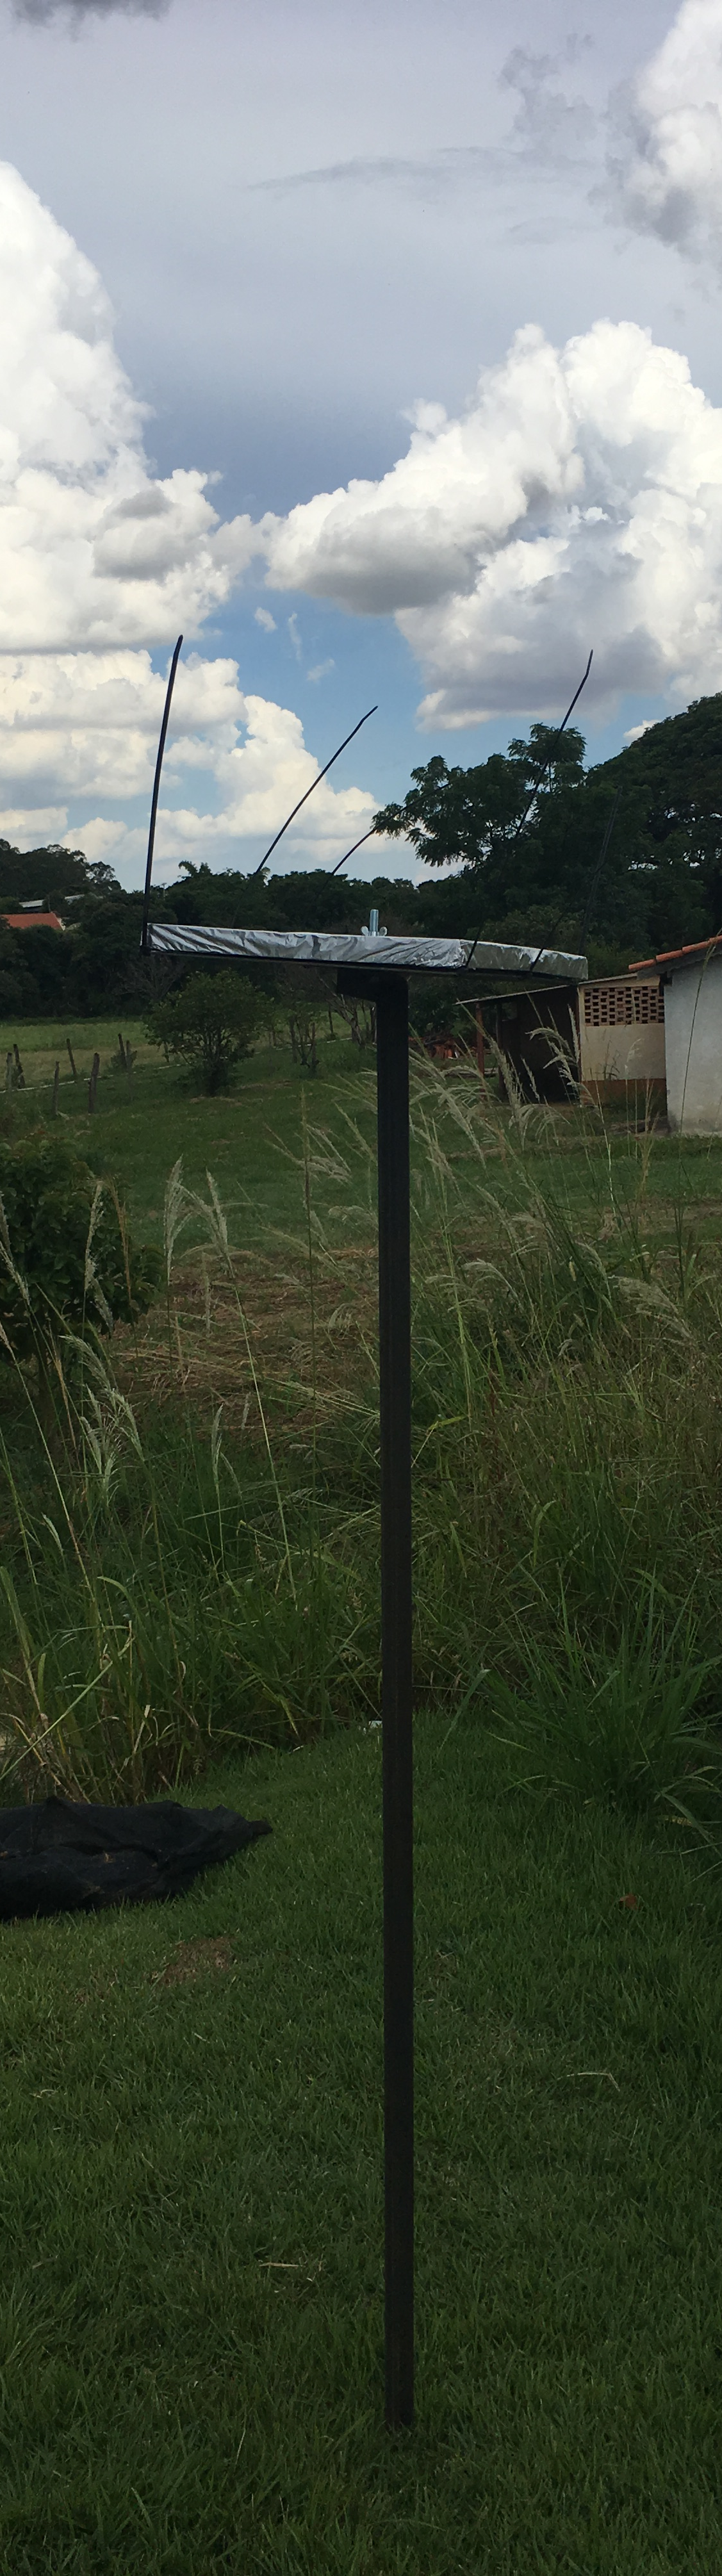
\includegraphics[width=0.158\columnwidth]{figs/hailpad.png}
			\label{hailpad_indaiatuba}}\\
		\legend{Fonte: Produzido pela autora.}
	\end{center}
\end{figure}

Os casos descritos na \autoref{tabela_casos} foram selecionados com base nos registros dos hailpads dentro da rede. A \autoref{tabela_hailpads} mostra a localização das placas e os grupos que mediram a distribuição de tamanho de granizo, sendo eles: Laboratório de Instrumentação Meteorológica (LIM/CPTEC-INPE) e Departamento de Ciências Atmosféricas (DCA/IAG-USP). Não houve registro da localização exata da placa C004. 

\begin{table}[htb]
	\IBGEtab{%
		\caption{Descrição dos hailpads coletados para cada caso.}%
		\label{tabela_hailpads}
	}{%
		\begin{tabularx}{\textwidth}{YYYY}
			\toprule
			Data do evento & Código do hailpad coletado & Localização & Medido por \\
			\midrule 
			2016-12-25 & C002 & Campinas & IAG, LIM \\
			\midrule 
			2017-01-31 & C003 & Campinas & IAG, LIM \\ 
			 & C004 & Arredores de Campinas & IAG, LIM \\
			\midrule 
			2017-03-14 & C001 & Cosmópolis & IAG \\ 
			& R002 & Indaiatuba & IAG \\
			\midrule 
			2017-11-15 & R004 & Indaiatuba & IAG \\
			\midrule 
			2017-11-16 & R038 & Campinas & IAG \\
			\bottomrule
		\end{tabularx}%
	}{%
		\fonte{Produzido pela autora.}%
	}
\end{table}

A partir de um hailpad é possível derivar diversas grandezas relacionadas à tempestade que gerou a queda de granizo. A principal delas é a distribuição de tamanho de granizo, medindo as cavidades na placa sensibilizada (\autoref{hailpad_exemplo}). Essa grandeza foi obtida através de uma série de medições manuais dos diâmetros das cavidades com um paquímetro e ajustando os dados com a curva de calibração desse tipo de isopor, realizada pelo LIM e exibida na \autoref{calibracao_hailpad}. Com essa distribuição, pode-se calcular a energia cinética do granizo (quando diversas placas mediram um mesmo evento) ou do hailpad (quando poucas ou uma única placa mediram um evento). Ambas grandezas são equivalentes ao trabalho mecânico sofrido pela superfície onde caiu o granizo, indicando então o dano causado por ele na superfície.

\begin{figure}[htb]
	\begin{center}
		\caption{Placa R004 sensibilizada no sítio (a) e sem a cobertura de alumínio (b).} 
		\label{hailpad_exemplo}
		\subfloat[]{\includegraphics[width=0.4\columnwidth]{figs/hailpad_site.jpg}
			\label{hailpad_sensibilizado}}
		\quad
		\subfloat[]{\includegraphics[width=0.357\columnwidth]{figs/hailpad_used.JPG}
			\label{hailpad_semaluminio}}\\
		\legend{Fonte: A autora.}
	\end{center}
\end{figure}

\begin{figure}[htb]
	\begin{center}
		\caption{Curva de calibração do hailpad obtida pelo LIM/CPTEC-INPE.} 
		\label{calibracao_hailpad}
%		\setcaptionmargin{1cm}
		\includegraphics[width=0.7\columnwidth]{figs/calibracao_hailpad.png}
		\legend{Fonte: \citeonline{ThomazJunior2015a}.}
	\end{center}
\end{figure}

Como houve no máximo 2 placas sensibilizadas em todos os casos, calculou-se a energia cinética da tempestade de granizo registrada no hailpad $E_t (Jm^{-2})$, definida por \citeonline{Mezeix1981} como:

\begin{equation}
	E_t = 4,58 e^{-6} \sum_{i=1}^{k} n_i d_i^4
\end{equation}

\noindent
sendo $n_i$ a quantidade de pontos por $m^2$ em um dado diâmetro médio $d_i (mm)$ de um intervalo $\Delta d$. $k$ é o numero de intervalos, igual a 9 nesse caso já que $\Delta d$ variou entre 2 e 22 mm com espaçamento de 1 mm. Foram consideradas incertezas nas medidas propagando o desvio-padrão da distribuição média entre as diferentes medidas de uma mesma placa.

Com os valores de diâmetro do granizo e energia cinética do hailpad, duas escalas que definem a intensidade de tempestades de granizo foram comparadas entre si. A \autoref{tabela_escalas} descreve as escalas ANELFA e TORRO, comparando-as de acordo com o descrito por \citeonline{Dessens2007}. A escala ANELFA, referente à organização que a desenvolveu (\textit{Association Nationale d’Etude et de Lutte contre les Fléaux Atmosphériques}, Associação para Suprimir Pragas Atmosféricas), foi desenvolvida na França usando uma série de 16 anos de dados de hailpads e compara o diâmetro máximo do granizo com a energia cinética do hailpad, indicando possíveis dados (principalmente a plantações) que um evento com dado tamanho de granizo pode causar \cite{Dessens2007}. O índice varia entre A0 (onde ocorre danos à folhas de árvores) e A5 (onde o evento é extremamente perigoso e pode causar mortes). A escala TORRO de intensidade de queda de granizo, também referente à organização que a desenvolveu (\textit{Tornado and Storm Research Organisation}, Organização de Pesquisa em Tornado e Tempestade), foi desenvolvida na Grã-Bretanha e compara o diâmetro típico (interpretado aqui como a mediana da distribuição) do granizo com a energia cinética e também indica possíveis danos que o evento pode causar \cite{webb1986}. Este índice varia entre H0 (onde não há danos) e H10 (onde há extensivos danos estruturais).

\begin{table}[htb]
	\IBGEtab{%
		\caption{Descrição das escalas ANELFA e TORRO, com comparação entre o dano típico de cada escala.}%
		\label{tabela_escalas}
	}{%
		\begin{tabularx}{\textwidth}{YcYcY}
			\toprule
			 & \multicolumn{2}{c}{ANELFA} & \multicolumn{2}{c}{TORRO} \\
			\midrule
			Objeto Equivalente ao Tamanho do Granizo & Escala & Dano Típico & Escala & Dano Típico \\
			\midrule
			Ervilha & A0 & Acidentes de trânsito, danos a folhas de árvores & H0 & Sem danos
\\
			\midrule 
			Naftalina & A1 & Danos a vinhas, pomares, tabaco & H1 & Danos gerais leves a plantas e plantações
 \\
			\midrule 
			Bola de Gude, Uva & A2 & Danos sérios a cereais, vegetais, árvores & H2 & Danos significativos a frutas, plantações e vegetações
\\
			\midrule 
			Noz & A3 & Danos totais a todas as plantações, vidros quebrados, carros danificados & H3 & Danos severos a frutas e plantações, danos a estruturas de vidro e plástico, pinturas em madeiras
\\
			\midrule 
			Ovo de Pombo a Bola de Squash & A4 & Paisagem de inverno, mortes de animais, pessoas feridas, danos a aviões pousados & H4 & Danos difundidos em vidros, danos em carrocerias de veículos
\\
			Bola do Golfe a Ovo de Franga & & & H5 & Destruição total de vidros, danos a telhados de azulejo, riscos significativos de ferimentos
\\
			\midrule 
			Ovo de Galinha & A5 & Evento extremamente perigoso, morte de pessoas desprotegidas & H6 & Carrocerias de aeronaves pousadas amassadas, paredes de tijolos furadas
\\
			Bola de Tênis a Bola de Cricket & & & H7 & Danos severos a telhados, risco de ferimentos sérios
\\
			Laranja Grande a Bola de Softball & & & H8 & (Evento mais severo registrado nas Ilhas Britânicas) Danos severos a aeronaves
\\
			Toranja & & & H9 & Danos estruturais extensivos; Risco de ferimentos severos ou até fatais em pessoas a céu aberto
\\
			Melão & & & H10 & Danos estruturais extensivos; Risco de ferimentos severos ou até fatais em pessoas a céu aberto \\
			\bottomrule
		\end{tabularx}%
	}{%
		\fonte{Adaptado de \citeonline{Dessens2007} e http://www.torro.org.uk/hscale.php.}%
	}
\end{table}


\section{Radares Meteorológicos}\label{radar}

A \autoref{cobertura_radares} mostra a localização e cobertura espacial dos radares utilizados neste trabalho. A \autoref{estrategia_radares} mostra a estratégia de varredura de cada radar.

\begin{figure}[htb]
	\begin{center}
		\caption{Localização e cobertura dos radares da FCTH (laranja), de São Roque (azul) e o XPOL (verde). As linhas mais grossas representam a cobertura de 250 (80) km dos radares FCTH e São Roque (XPOL), enquanto que as linhas mais finas representam a cobertura de 100 (60) km dos mesmos radares.} 
		\label{cobertura_radares}
		\includegraphics[width=\columnwidth]{figs/radar_coverages_hires2.jpg}
		\legend{Fonte: Produzido pela autora.}
	\end{center}
\end{figure}

O radar Doppler Banda-S de dupla polarização operado pela Fundação Centro Tecnológico de Hidráulica (FCTH) é localizado na barragem de Ponte Nova, município de Biritiba Mirim (23\textdegree36’S, 45\textdegree58’20’’W, 916 m de altitude). Este radar faz uma varredura volumétrica a cada 5 minutos em uma cobertura de até 250 km, com 8 elevações (1\textdegree, 1,6\textdegree, 2,4\textdegree, 3,2\textdegree, 4,2\textdegree, 5,5\textdegree, 6,9\textdegree e 8,6\textdegree) de 1\textdegree de abertura do feixe, como mostra a Figura\autoref{estrategia_cth}. Os dados volumétricos foram convertidos em uma grade de 1 x 1 x 1 km usando o pacote Py-ART (\textit{Python ARM Radar Toolkit}, Conjunto de Ferramentas de Radar em Python do ARM) \cite{Helmus2016} e perfis horizontais (em 3 km de altura) e verticais (cortes entre dois pontos com coordenadas latitudinais e longitudinais) foram analisados. Além da variável refletividade do radar, três variáveis polarimétricas foram analisadas e relacionadas com diferentes tipos de hidrometeoros seguindo a classificação de \citeonline{Straka2000} descrita na \autoref{hid}:

\begin{alineas}
	\item \textbf{Refletividade Diferencial}: Razão entre os fatores de refletividade horizontal e verticalmente polarizados; diferencia a forma das partículas em um dado volume medido;
	\item \textbf{Fase Diferencial Específica}: Calculada a partir das matrizes de espalhamento vertical e horizontal, é fortemente influenciada pela concentração numérica e massa de gotículas de nuvem, permitindo a derivação da distribuição de tamanho das mesmas;
	\item \textbf{Coeficiente de Correlação}: Razão entre as amplitudes das matrizes de espalhamento; destaca misturas de formas e tamanhos das partículas \cite{Rauber2018}.
\end{alineas}

O radar Doppler Banda-S operado pelo DECEA (Departamento de Controle do Espaço Aéreo) instalado em São Roque (23\textdegree35’56’’S, 47\textdegree5’52’’W, 1147,54 m de altitude) faz varreduras a cada 10 minutos em uma cobertura de até 250 km, com 15 elevações (0,5\textdegree, 1\textdegree, 2\textdegree, 3\textdegree, 4\textdegree, 5\textdegree, 6\textdegree, 7\textdegree, 8\textdegree, 9\textdegree, 10\textdegree, 12\textdegree, 14\textdegree, 16\textdegree e 18\textdegree) de 2\textdegree de abertura do feixe, como mostra a Figura\autoref{estrategia_sr}. Os perfis horizontais de CAPPIs (\textit{Constant Altitude Plan Position Indicator}, Indicador Plano de Posição em Altitude Constante) em 3 km de altura serviram como dados de entrada para o algoritmo ForTraCC (\textit{Forecast and Tracking the Evolution of Cloud Clusters}, Prevendo e Rastreando a Evolução de Aglomerados de Nuvens) \cite{Vila2008} adaptado para radares meteorológicos, rodado com limiar de refletividade de 35 dBZ.

O ciclo de vida da tempestade associada a cada caso foi definido a partir do sistema convectivo com maior intensidade na posição do hailpad, considerando o horário aproximado da queda de granizo. A partir desse sistema, a família - definição do algoritmo para um conjunto de sistemas próximos uns aos outros com mesmo deslocamento - associada a ele foi extraída e corrigida caso houvesse necessidade. A partir de cada rastreamento, variáveis como refletividade máxima e tamanho do sistema foram analisadas, além de servirem como base para a seleção de descargas elétricas associadas aos sistemas.

O radar Doppler Banda-X de dupla polarização XPOL foi operado pelo Projeto SOS-CHUVA na UNICAMP, cidade de Campinas (22\textdegree48’50’’S, 47\textdegree3’22’’, 680 m de altitude). Ele fez varreduras volumétricas a cada 10 minutos em uma cobertura de até 80 km, com 17 elevações (0,5\textdegree, 1,8\textdegree, 3,1\textdegree, 4,4\textdegree, 5,7\textdegree, 7\textdegree, 8,3\textdegree, 9,6\textdegree, 10,9\textdegree, 13\textdegree, 15\textdegree, 18\textdegree, 22\textdegree, 26\textdegree, 32\textdegree, 40\textdegree e 55\textdegree) de 1,3\textdegree de abertura do feixe, como mostra a Figura\autoref{estrategia_xpol}. Os dados volumétricos também foram convertidos em uma grade de 1 x 1 x 1 km e as variáveis refletividade do radar e velocidade radial foram utilizadas. Devido à falta de dados em muitos dos casos selecionados, este radar foi usado apenas como entrada no algoritmo de recuperação de vento por Multi-Doppler (\autoref{multidoppler}) juntamente com os demais radares.

\begin{figure}[htb]
	\begin{center}
		\caption{Estratégia de varredura volumétrica dos radares meteorológicos da FCTH (a), de São Roque (b) e o XPOL instalado na UNICAMP (c).} 
		\label{estrategia_radares}
		\subfloat[]{\includegraphics[width=0.75\columnwidth]{../General_Processing/figures/scan_strategy_cth.png}\label{estrategia_cth}}\\
		\subfloat[]{\includegraphics[width=0.75\columnwidth]{../General_Processing/figures/scan_strategy_sr.png}\label{estrategia_sr}}\\
		\subfloat[]{\includegraphics[width=0.75\columnwidth]{../General_Processing/figures/scan_strategy_xpol.png}\label{estrategia_xpol}}\\
		\legend{Fonte: Produzido pela autora.}
	\end{center}
\end{figure}

\subsection{Identificação de Hidrometeoros}\label{hid}

\begin{figure}[htb]
	\begin{center}
		\caption{Classificação de hidrometeoros de acordo com refletividade (a), refletividade diferencial (b), fase diferencial específica (c) e coeficiente de correlação (ou razão de correlação cruzada) (d).} 
		\label{hid_straka}
%		\setcaptionmargin{1cm}
		\includegraphics[width=\columnwidth]{../General_Processing/figures/hids_strakaetal.png}
		\legend{Fonte: Produzido pela autora a partir de \citeonline{Straka2000}.}
	\end{center}
\end{figure}


\subsection{Recuperação de Vento por Multi-Doppler}\label{multidoppler}

\begin{figure}[htb]
	\begin{center}
		\caption{Ângulos teóricos de cruzamento do feixe com Dual-Doppler de 45\textdegree (melhores dados de vento) e 30\textdegree (dados de vento aceitáveis) para um par de radares Doppler, mais especificamente para as combinações dos radares FCTH e XPOL, São Roque (SR) e FCTH e SR e XPOL. Os contornos em cinza representam as cidades de São Paulo, Indaiatuba e Campinas, enquanto que as linhas pontilhadas indicam as distâncias entre os radares.} 
		\label{doppler_lobes}
		%		\setcaptionmargin{1cm}
		\includegraphics[width=0.65\columnwidth]{../General_Processing/figures/dual_doppler_lobes.png}
		\legend{Fonte: Produzido pela autora.}
	\end{center}
\end{figure}


\section{Rede de Detecção de Raios}\label{raios}

\subsection{Conversão Strokes-Flashes}\label{strokestoflashes}

